\documentclass[a4paper 12pt]{article}

\usepackage[utf8]{inputenc}
\usepackage[T1]{fontenc}
\usepackage{mathptmx}
\usepackage{textcomp}
\usepackage[UKenglish]{babel}
\usepackage{amsmath, amssymb}
\usepackage{float}
\usepackage[hidelinks]{hyperref}
\hypersetup{
	colorlinks=false
}
\usepackage[style=ieee]{biblatex}
\bibliography{sources/biblio}
\renewcommand{\baselinestretch}{1.5}

\setlength{\parindent}{0pt}
\setlength{\parskip}{1em}

% figure support
\usepackage{import}
\usepackage{xifthen}
\pdfminorversion=7
\usepackage{pdfpages}
\usepackage{transparent}
\newcommand{\incfig}[1]{%
	\def\svgwidth{\columnwidth}
	\import{./figures/}{#1.pdf_tex}
}

\pdfsuppresswarningpagegroup=1

\begin{document}
\begin{titlepage}
  \begin{center}

    \textsc{\LARGE Dublin City University}\\[1cm]
    \textsc{\Large Electronic and Computer Engineering}\\[0.5cm]

    {\LARGE \bfseries EE515 Real-Time DSP: Assignment 1\\[0.4cm]}
    {\Large \bfseries The role of Digital Signal Processing in Optical
    Communications Systems\\[0.4cm]}

    \begin{figure}[H]
	
\includegraphics{images/Dcu-logo.png}
	\centering
    \end{figure}

    \vskip 2cm
    \emph{Author}\\[0.1cm]
    \noindent\makebox[\textwidth]{%
      \begin{tabular}{ll}%
        Michael Lenehan & michael.lenehan4@mail.dcu.ie \\
	Student Number: & 15410402 \\
    \end{tabular}}\\[0.1cm]

    \vfill

    % Bottom of the page
    % Probably replaced with date of deadline
    {\large{26/11/2019}}

  \end{center}
\end{titlepage}

\thispagestyle{plain}
\begingroup
\renewcommand{\cleardoublepage}{}
\renewcommand{\clearpage}{}

\LARGE{Declaration}

\endgroup

\vskip 1cm

I declare that this material, which I now submit for assessment, is entirely my
own work and has not been taken from the work of others, save and to the extent
that such work has been cited and acknowledged within the text of my work. I
understand that plagiarism, collusion, and copying are grave and serious
offences in the university and accept the penalties that would be imposed should
I engage in plagiarism, collusion or copying. I have read and understood the
Assignment Regulations set out in the module documentation. I have identified
and included the source of all facts, ideas, opinions, and viewpoints of others
in the assignment references. Direct quotations from books, journal articles,
internet sources, module text, or any other source whatsoever are acknowledged
and the source cited are identified in the assignment references. This
assignment, or any part of it, has not been previously submitted by me or any
other person for assessment on this or any other course of study.

I have read and understood the DCU Academic Integrity and Plagiarism at
\url{https://www4.dcu.ie/sites/default/files/policy/1%20-%20integrity_and_plagiarism\_ovpaa_v3.pdf}
and IEEE referencing guidelines found at
\url{https://loop.dcu.ie/mod/url/view.php?id=448779}.

\vskip 1cm
Signed: \underline{\ \ \ \ \ \ \ \ \ \ \ \ \ \ \ \ \ \ \ \ \ \ \ \ \ \ \ \ \ \ \ \ \ \ \ \ \ } \hspace{20mm}Date: \underline{08/04/2019}

\hspace*{0mm}\phantom{Signed:}Michael Lenehan

\pagebreak

\thispagestyle{plain}
\begin{center}
    \Large
    \textbf{EE-515 Real-Time DSP Assignment 1}

    \vspace{0.4cm}
    \large
    The role of Digital Signal Processing in Optical Communications Systems

    \vspace{0.4cm}
    \textbf{Michael Lenehan}

    \vspace{0.9cm}
    \textbf{Abstract}
\end{center}
\pagebreak

\tableofcontents
\clearpage
\section{Introduction}
Modern optical communications systems have been in use since the 1960's, with
the first commercial usage in 1977 in California, where telephone traffic was
transmit at a rate of 6Mbps\cite{alwayn_2004}. Since this time, systems have
been implemented to transmit data for applications such as telephony, cable
television, and internet data.
\par This literature review will present a history of the usage and
implementations of optical communications systems, and an overview of the
applications of the technology.
\par Following this, a review of the current ``state of the art'' within the
field, as it applies to digital signal processing, and the modulation algorithms
implemented, will be completed.

\section{Background}
In order to understand the ``state of the art'' within the field of optical
communications systems with relation to digital signal processing, it is
necessary to have a level of understanding of its background. This section will
introduce the basic physics concepts, a generalised overview of a typical
optical communications system, along with the advantages an optical
communication system offers.

\subsection{The Physics of Optical Communications}

Optical communications systems utilise light, typically provided by laser
diodes, or LED's, in order to transmit information along an optical fiber cable.
The optics principle of total internal reflection is utilised for the purpose of
transmission. When the incident angle of the light in the cable is greater than
the critical angle at the ``core-to-cladding interface''\cite{alwayn_2004}, the
light will reflect back into the core. This repeats thoughout the fibers core,
passing the light from source to destination.

\begin{figure}[H]
	\centering
	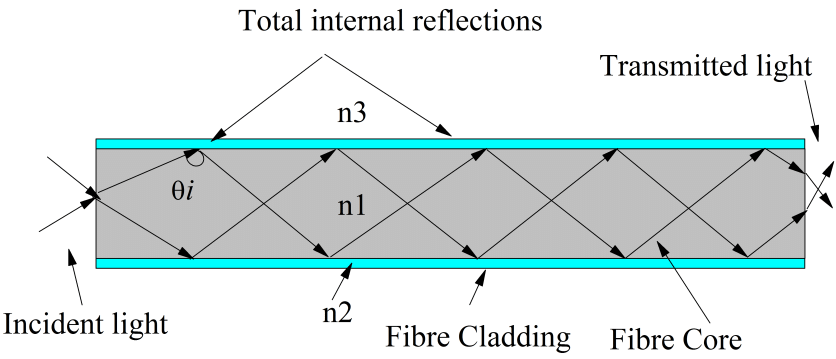
\includegraphics[width=0.8\textwidth]{images/tir}
	\caption{Total Internal Reflection within an Optical Fiber
	Cable\cite{memon_2018}}
	\label{fig:tir}
\end{figure}

\par Optical communications systems utilise light in the infrared spectrum to pass
information along a cable. The wavelength of the light in this spectrum is
in the order of thousands of micrometers ($\mu m$) in length, with frequencies
in the order of hundreds of terahertz ($\approx 10^{13}Hz$). These
high-frequency, low-wavelength carrier signals result in very high bandwidths,
and very high data transfer rates\cite{mickelson_2003}.

\par The directionality of laser light within these systems allows for greater
efficiency, as energy is not required for the filtering or correction of
divergent beams\cite{mickelson_2003}.

\subsection{Optical Communications System Overview}

Optical communications systems are typically composed of the components listed
in figure \ref{fig:overview}, that is a light source, an information source, an
encode and modulator, optics at both the transmitting and receiving side, a
transmission medium, a detector, and a receiver.

\begin{figure}[H]
	\centering
	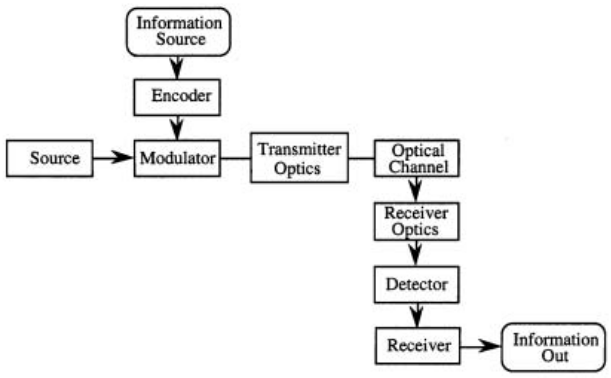
\includegraphics[width=0.8\textwidth]{images/optcommsblock}
	\caption{Generalised Block Diagram of an Optical Communications System
	\cite{mickelson_2003}}
	\label{fig:overview}
\end{figure}

\par As previously discussed, the light source used is typically an LED or a laser
diode (LD). Laser diodes offer advantages in modulation speed, power and spatial
coherence\cite{alwayn_2004}.

\par At the transmission side, the incoming source must be modulated with the data
signal. The modulation techniques used, and the most recent advances in these
techniques will be the main focus of this review paper.

\par At the receiving side, a photodiode converts the incoming light signal to
an electrical signal. This is typically followed by multiple amplication stages,
and can also include circuitry for decoding the signal, or error
detection\cite{alwayn_2004}.

\subsection{Optical Communications System Advantages}

There are many advantages to using optical communications systems over
traditional communications systems using, for example, copper wire. Optical
communications systems allow for greater resistance to interference and signal
attenuation, which can cause problems in traditional systems.

\subsubsection{Interference}

Interference can be present in traditional data transmissions through a
phenomenon known as ``Crosstalk'' which occurs when signals within different
channels of a system have an adverse, interfering effect on one
another\cite{wikipediacross_2019}. While this is an issue within the traditional
data communications systems, limiting the amount of lines which can be run in
close proximity, it poses no such issues within optical communication systems
(provided there is adequate cladding in place\cite{mickelson_2003}).

\par Optical data transmission is relatively resistant to interference, both in
terms of Electromagnetic, and Radio-Frequency interference, thus making them
more suitable than metal based, traditional transmission systems in situations
where there is high likelihood of these types of interference\cite{alwayn_2004}.

\subsubsection{Attenuation}

Attenuation in optical systems is much less of an issue than in its metal based
counterpart. This is due to attenuation being mainly caused by absorption and
scattering within the transmission medium\cite{alwayn_2004}. Within glass cable,
this attenuation is extremely low, however, with plastic core cable, it can be
higher, due to impurities within the material\cite{alwayn_2004}.

\par Attenuation within traditional systems is higher due to the ``skin effect''
which increases attenuation at higher frequencies\cite{hayt_buck_2019}. Due to
this effect, systems utilising copper wire require repeaters at approximately
2-5km intervals, compared to a distance of approximately 50km in fiber optic
cabling\cite{mickelson_2003}\cite{fiber_vs_wire}.

\section{Current}
\subsection{Modulation Techniques}

Currently there is a body of work being produced within the area of modulation
techniques for optical communications systems. One such technique, showing
promise in increasing spectral efficiency\cite{prob_2016}, while simultaneously
achieving lower optical signal to noise ratios (OSNR), and higher transmissions
distances\cite{400Gbps_2019}, is Probabilistic Shaping.

\section{Conclusions}
It is clear that there has been much work done on modulation techniques, signal
recovery, and coherent detection within the last number of years. These
techniques have allowed for benefits such as offsetting noise introduced in
transmission, reducing system complexity, increasing transmission distances, and
increase in performance.

\par While newer machine learning techniques are promising increased
performance, on lower cost, lower power ADC's, there is still work being done on
increasing performance to the greatest extent possible using more traditional
DSP techniques, as with probabilistic shaping.

\par The aim of all of the techniques mentioned is to increase data rates and
throughput within optical communications systems in an effort to increase their
usage and ubiquity in worldwide communication systems.

test \cite{5367579}
\clearpage
\printbibliography
\end{document}
